\chapter{Introducción}

\section{Motivación}

Alicia y Roberto forman un matrimonio de muchos años
al igual que sus amigos Marcelo y Beatriz. Con el pasos de los años
ambos matrimonios han ido perdiendo la fuerza y la rutina ha ido socabando
la pasión que alguna vez existió. Es así como Alicia decidió iniciar una
aventura con el marido de su amiga Beatriz, Marcelo, y coincidentemente
Beatriz decidio hacer lo mismo con el marido de su amiga.\\
Hace algún tiempo Alicia comenzó a tomar un curso básico de computación donde
ha aprendidio a \textit{chatear} y, como Carlos ha caído postrado en la cama por
enfermedades asociadas a su avanzada edad, ha enseñado a sus amigos a chatear para
``poder comunicarse sin tener que salir de casa". Pero esto no es más que una fachada
para encubrir su engaño (y sin querer encubirir el de Beatriz también), pues Alicia
quiere desea declararse \textit{on-line} con Marcelo y de paso lo mismo hará Beatriz
con Roberto.\\
Alicia, temerosa de ser descubierta y con ayuda del curso de computación, se ha dado
cuenta de que cualquiera podría descubrir su infidelidad viendo cuales son los paquetes
intercambiados entre el computador de Marcelo y ella. También ha estado pensando paranoicamente
que Roberto podría estar tomando un curso de \textit{hacker} en la municipalidad y podria
intentar hacerse pasar por Marcelo e interferir en sus conversasiones privadas. Lo último que
preocupa a Alicia es la influencia que pueden tener los otros programas que ejecutan el computador
de ella o el de sus amigos.\\
Alicia ha determinado que su problema es exacatamente el siguiente:\\
\textit{Desea crear un protocolo  en el que la comunicación es anonima y
además es imoposible que alguien impersone a otro. Adicionalmente Alicia desea que las garantías
anteriores se mantengan inclusive si el protocolo es ejecutado concurrentemente con otros protocolos}\\ 
En esta memoria se desarrollará un protcolo criptográfico y se demostrará rigurosamente que cumple con
las garantías necesaria para solucionar el problea anterior, utilizando herramientas modernas de Criptografía. 

\section{Descripción del problema}

En general el problema anterior puede a aplicarse a cualquier de grupo de personas que
desea comunicarse entre sí en una red (internet o una red local) y desea obtener garantías
similares. A continuación iniciamos el camino de formalización del problema motivacional.\\
La solución del problema consiste en encontrar un protocolo (un algoritmo distribuido) de cual
se puedan garantizar matemáticamente las siguientes tres propiedades :
\begin{enumerate}
    \item Anonimato
    \item Autentificación desmentible
    \item Componibilidad
\end{enumerate}

\subsubsection{Anonimato}
A modo de ejemplo podemos considerar un protocolo ``usual" de comunicación, un protcolo IP simplificado.
En la figura \ref{tcpip_simple} la figura cada flecha de $A$ a $B$ indica que $A$ envió un mesaje a
$B$. La etiqueta de una flecha de $A$ a $B$ indica el mensaje intercambiados en la ejecución de protocolo.
Por ejemplo Roberto envió a Alicia el mensaje $(m_{AR}, ip_R, ip_A)$, donde $m_{AR}$ es el contenido
del mensaje, $ip_R$ es la dirección IP de Roberto y $ip_A$ es la dirección IP de Alicia. Notemos que estos
datos son necesarios para poder \textit{rutear} los mensajes de un participante a otro, pero a la vez 
revelando a un adversario que Roberto envio un mensaje a Alicia. Por lo tanto podemos decir que
\textbf{el protocolo IP simplificado no es anónimo} pues \textbf{existe un ataque}.\\

\begin{figure}[hp]
    \centering
    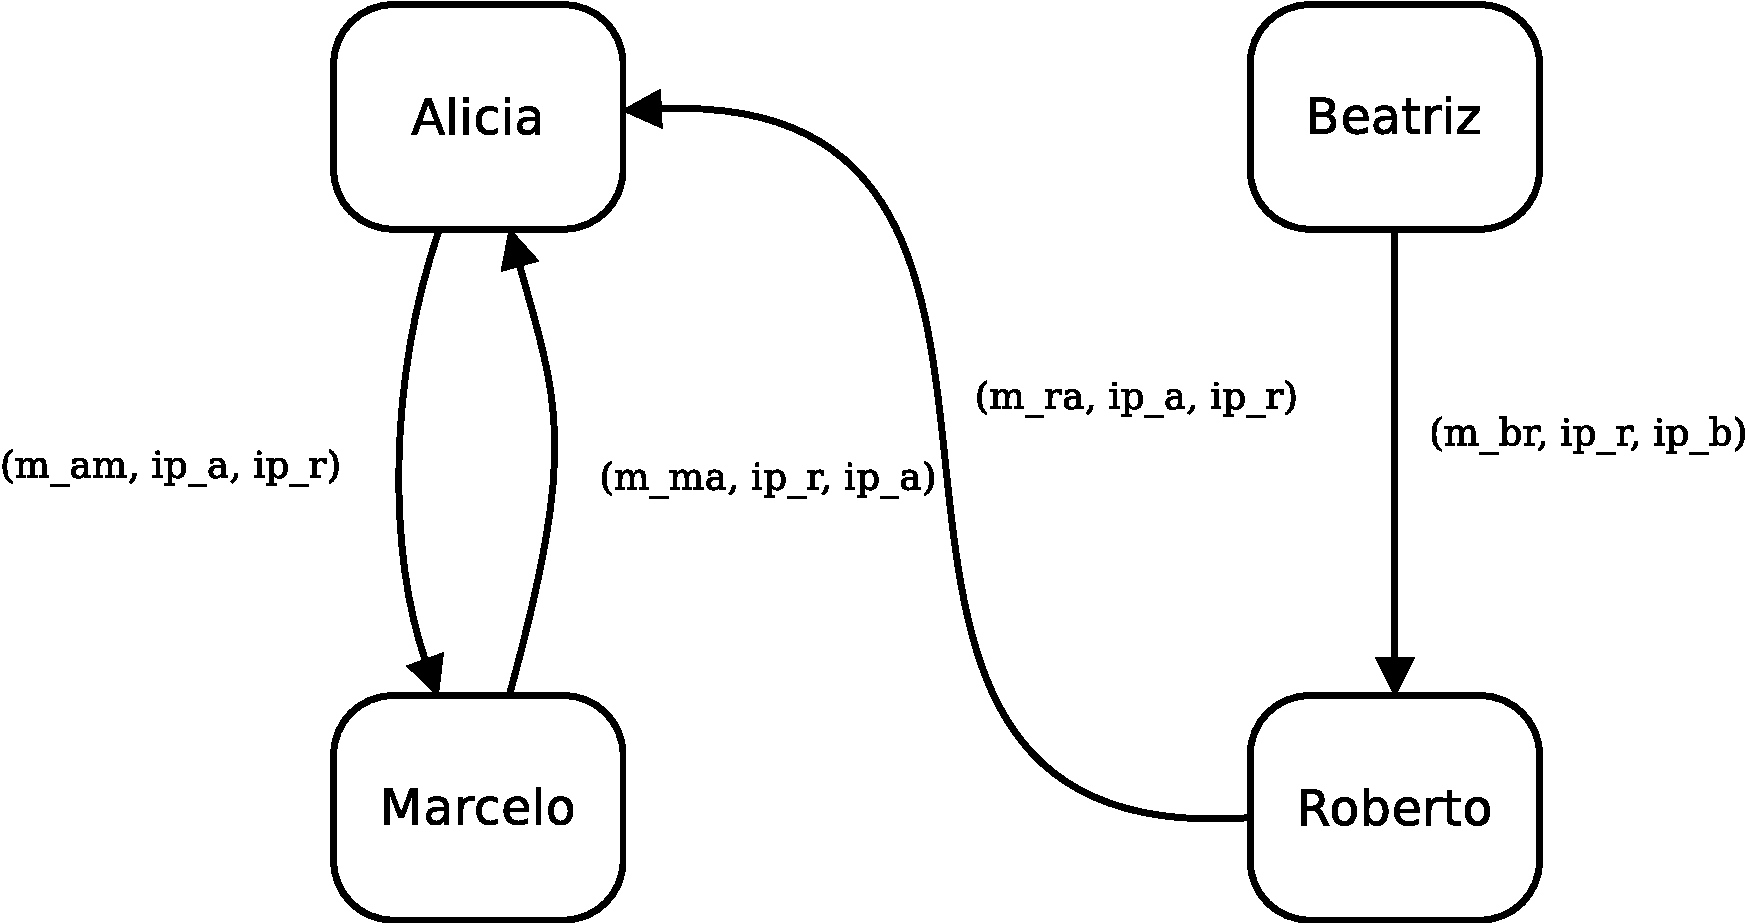
\includegraphics[width=0.7\textwidth]{figs/tcpip_simple}
    \caption{Protocolo simple de comunicación}
    \label{tcpip_simple}
\end{figure}

Para definir el anonimato resulta crucial definir formalmente que es considerado
un ataque al anonimato, pues un protocolo será anónimo si y solo si no existe ningún ataque.
En \cite{conf/pet/HeviaM08} se define un ataque con el siguiente juego.
El adversario determinada dos posibles ejecuciones del protocolo, las cuales difieren en
qué mensajes seran enviados por quién y qué mensajes fueron recibidos por quién. Entonces
consideraremos que el adversario realiza un ataque si al ejecutar al adversario con cada una
de las posibles ejecuciones del protocolo, el adversario logra identificar cuál es.
Por lo tanto un protocolo sera seguro si y solo si cualquier adversario no logra distinguir
una ejecución de otra.

\subsubsection{Autentificación desmentible}
En el procolo de la figura \ref{tcpip_simple} es posible que un adversario (rol que podria ser
tomado por Marcelo) se haga pasar por Beatriz e intente comunicarse con Alicia, y para ello
solo es necesario que modifique los mensajes uno de sus mensajes cambiando $ip_M$ por $ip_B$.
Por lo tanto decimos que el protocolo no implementa canales autenticados.\\
Con canales autentificado nos referimos protocolos en los cuales es posible estar seguro,
con alta probabilidad, de quién es el autor de un mensaje. Sin embargo hay que ser cuidadoso
con el protocolo de autentificación usado, pues los más conocidos
(firmas digitales por ejemplo) poseen la propiedad de \textit{non repudiability}. Esto es
que el emisor de un mesaje autentificado no puede negar a ``la comunidad" que el es el autor
del mensaje. Esto estaría contradiciendo el anonimato, pues el adversario también sería capaz
de asociar la autoria de un mensaje a el emisor de este.\\
La autentificacion desmentible, introducida en \cite{DwoNaoSah04}, se refiere a los protocolos
que implementan canales anónimos con la propiedad adicional de que cada mensaje es autentificado
a un receptor específico y el receptor no es capaz de probar a nadie más quién es el autor del mensaje.

\subsubsection{Componibilidad}
En general el hecho de implementar protocolos con ciertas garantías (por ejemplo anonimato y
autentificación desmentible) no garantiza que dichas propiedades se sigan teniendo cuando
el protocolo es ejecutado concurrentemente con otros protocolos.\\
En \cite{conf/focs/Canetti01} Canetti introduce el \textit{framework} criptografico conocido
como \textit{Universal Composabillity} (desde ahora UC). UC propone una metodología definir y
demostrar los objetivos de seguridad de un protocolo (por ejemplo anonimato y autentificación)
de un protocolo. UC garantiza que el protocol mantendrá su seguridad inclusive
si es ejecutado concurrentemente con cualquier protocolo, siempre y cuando no comparta estado
con el protocolo analizado.\\
Cuando el protocolo sí comparte estado con otros protocolo es necesario hacer uso del
\textit{framework Generalized Universal Composabillity} (desde ahora GUC), que generaliza a UC.
Informalmente GUC propone una metodología para incluir el estado que un protocolo podría compartir
con otros.

\subsubsection{Solución propuesta}
En esta memoria proponemos un protocolo que permite solucinar nuestro problema motivacional
utilizando técnicas de Anonimato y Autentificación desmentible y demostramos que el protocolo
resuelve el problema utilizando el \textit{framework} GUC. Es decir el protocolo soluciona
el problema inclusive si es ejecutado concurrentemente con otros protocolos que pueden compartir
estado con él.\\
En la figura \ref{sigmix_simple} se muestra un diagrama para explicar nuestra solución.

\begin{figure}[hp]
    \centering
    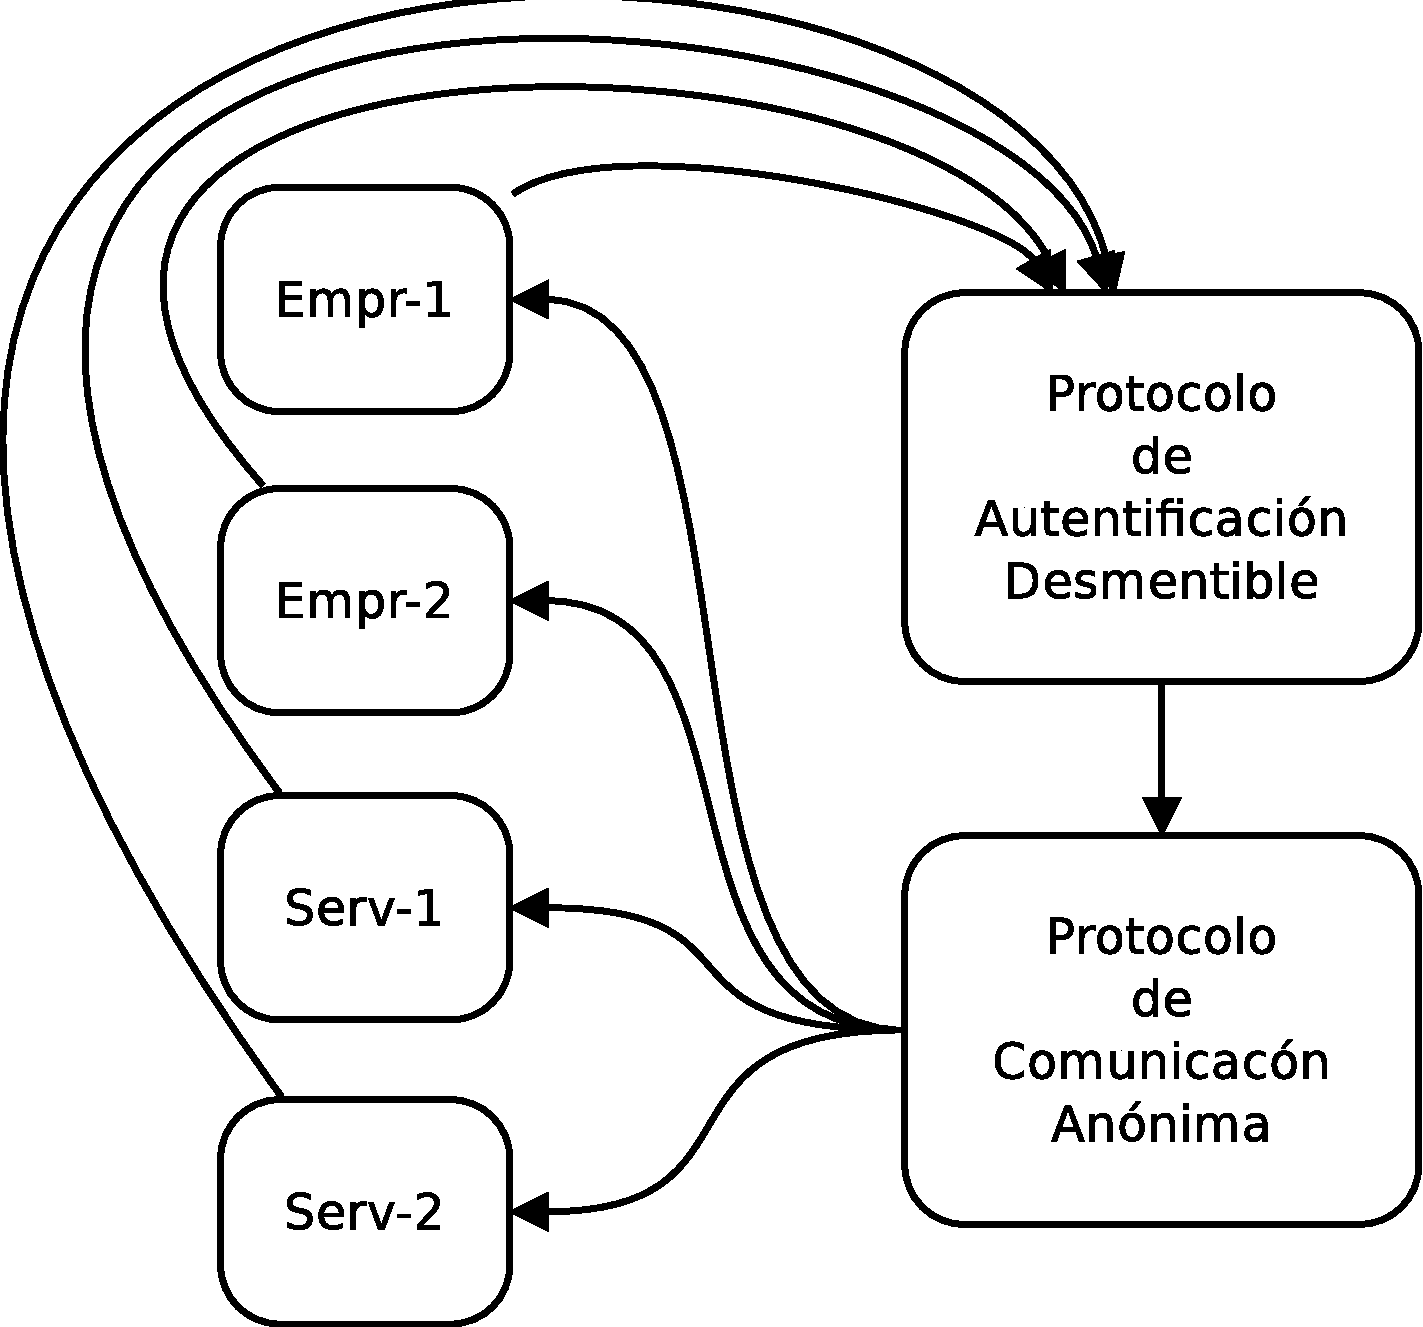
\includegraphics[width=0.5\textwidth]{figs/sigmix_simple}
    \caption{Solución propuesta}
    \label{sigmix_simple}
\end{figure}

